%!TEX root = main.tex
\section{The Sensemaking Model for VQSs\label{sec:sensemaking}}
\change{
  To convey how the features in \zvpp addresses the analytical needs posed by each domain, we organize our PD findings into a sensemaking framework for VQSs. In this section, we first describe the space of problems addressable by VQSs. Then, as shown in Figure~\ref{fig:taxonomy}, we develop a taxonomy for organizing VQS capabilities into three sensemaking processes. From top to bottom, we first describe the design objectives of each sensemaking process, then we outline the design challenge addressed by each of the functional components that supports the sensemaking process. The mapping between specific \zvpp features and these functional components and sensemaking processes can be found in Table~\ref{bigfeaturetable}.
}
 %Starting from the bottom level of the taxonomy, we first describe what each component in our taxonomy encompasses, then we proceed onto the upper level of the taxonomy, .
%We first describe features that we incorporated into our enhanced VQS, \zvpp, thematically organized by components (grouping features in the bottom-most level to components in the second level of Figure~\ref{fig:taxonomy}).
%collaboratively-designed
%Next, we describe features that we incorporated into our enhanced VQS, \zvpp, thematically organized by component. Then, we introduce a taxonomy for organizing these components into three sensemaking processes, spanning different problem areas that VQSs are aimed to solve.
%\change{In this section, we will first introduce a taxonomy for organizing these components into}
%Based on feature requests and discussion with our participants, we incorporated key features missing in our original VQS.
%From these discussion and analysis of past VQSs, we identify nine components of VQSs, described below. T
% Along with analysis of past literature, we develop a taxonomy of key functionalities in VQSs.
% novel contribution on  ---
% contribute to holistic understanding on how sensemaking --- in VQS.
% study on how users
% Implication ---
% •	What types of questions/ dataset/ problem challenges are asked to VQS or can be addressed by VQS? (S3)
% •	What kind of features needs to be designed to address these challenges (S4 PD)
%We employed participatory design with our scientists to incorporate key features missing in our original VQS, and unaddressed in their existing workflows. From these discussion and analysis of past VQSs, we identify nine components of VQSs, described below.
\subsection{Characterizing the Problem Space for VQSs}
%Based on example use cases and feature components from participatory design, we further characterize the design space of VQSs. further characterize three sensemaking process within the problem space of VQSs.
%Given our earlier description of VQS features organized into components, we
\change{We now} introduce the three sensemaking processes by characterizing how they fit into different problem areas that VQSs are aimed to solve. Visual querying often consists of searching for a desired pattern instance (Z) across a visualization collection specified by some given attributes (X,Y). Correspondingly, we introduce two axes depicting the amount of information known about the visualized attribute and pattern instance.%, as shown in Figure~\ref{2dmodel}.
%(e.g., only interested in patterns related to a specific gene)
\par Along the \textbf{pattern instance} axis,
the visualization that contains
the desired pattern may already be \texttt{known} to the analyst,
exist as a pattern \texttt{in-the-head} of the analyst,
or \change{be} completely \texttt{unknown} to the analyst.
In the \texttt{known} pattern instance region (Figure~\ref{2dmodel} grey), visualization-at-a-time systems such as Tableau,
where analyst manually create and examine each visualization one at a time,
is more well-suited than VQSs, since analysts can directly work with the selected instance without the need for visual querying.
Inspired by Pirolli and Card's information
foraging framework~\cite{Pirolli}, which distinguishes
between information processing tasks that are \textit{top-down}
(from theory to data) and \textit{bottom-up} (from data to theory),
we define \textit{top-down pattern search} as \change{the process where analysts query a fixed collection of visualizations based on their in-the-head pattern (Figure~\ref{2dmodel} blue)}. On the other hand, \change{\textit{bottom-up
data-driven inquiries} (Figure~\ref{2dmodel} green) are driven by recommendations or queries that originate from the data (or equivalently, the visualization), since the pattern of interest is unknown and external to the user.} As we will discuss later, this process is crucial but underexplored in past work on VQSs.
%analysts often do not start with a known pattern instance. T
\par The second axis, \textbf{visualized attributes},
depicts how much the analyst
knows about which X and Y axes
they are interested in visualizing.
In both the astronomy and genetics use cases,
as well as past work in this space, \change{the attribute to be visualized is \texttt{known}, as data was in the form of a time series.} In the case of our material science participants, they wanted to explore relationships between different
X and Y variables. In this realm of \texttt{unknown} attributes, context creation (Figure~\ref{2dmodel} yellow) is
essential for allowing users to pivot across different visualization collections.%subspaces. %Most past VQSs assume that the analyst has a desired pattern in-the-head that could be conveyed through visual specification, such as a sketch.%---i.e., setting the stage for bottom-up or top-down processes---\dor{this clause is awkward?}% data was in the form of a time series % with \texttt{known} visualized attributes.
\begin{figure}[h!]
  \centering
  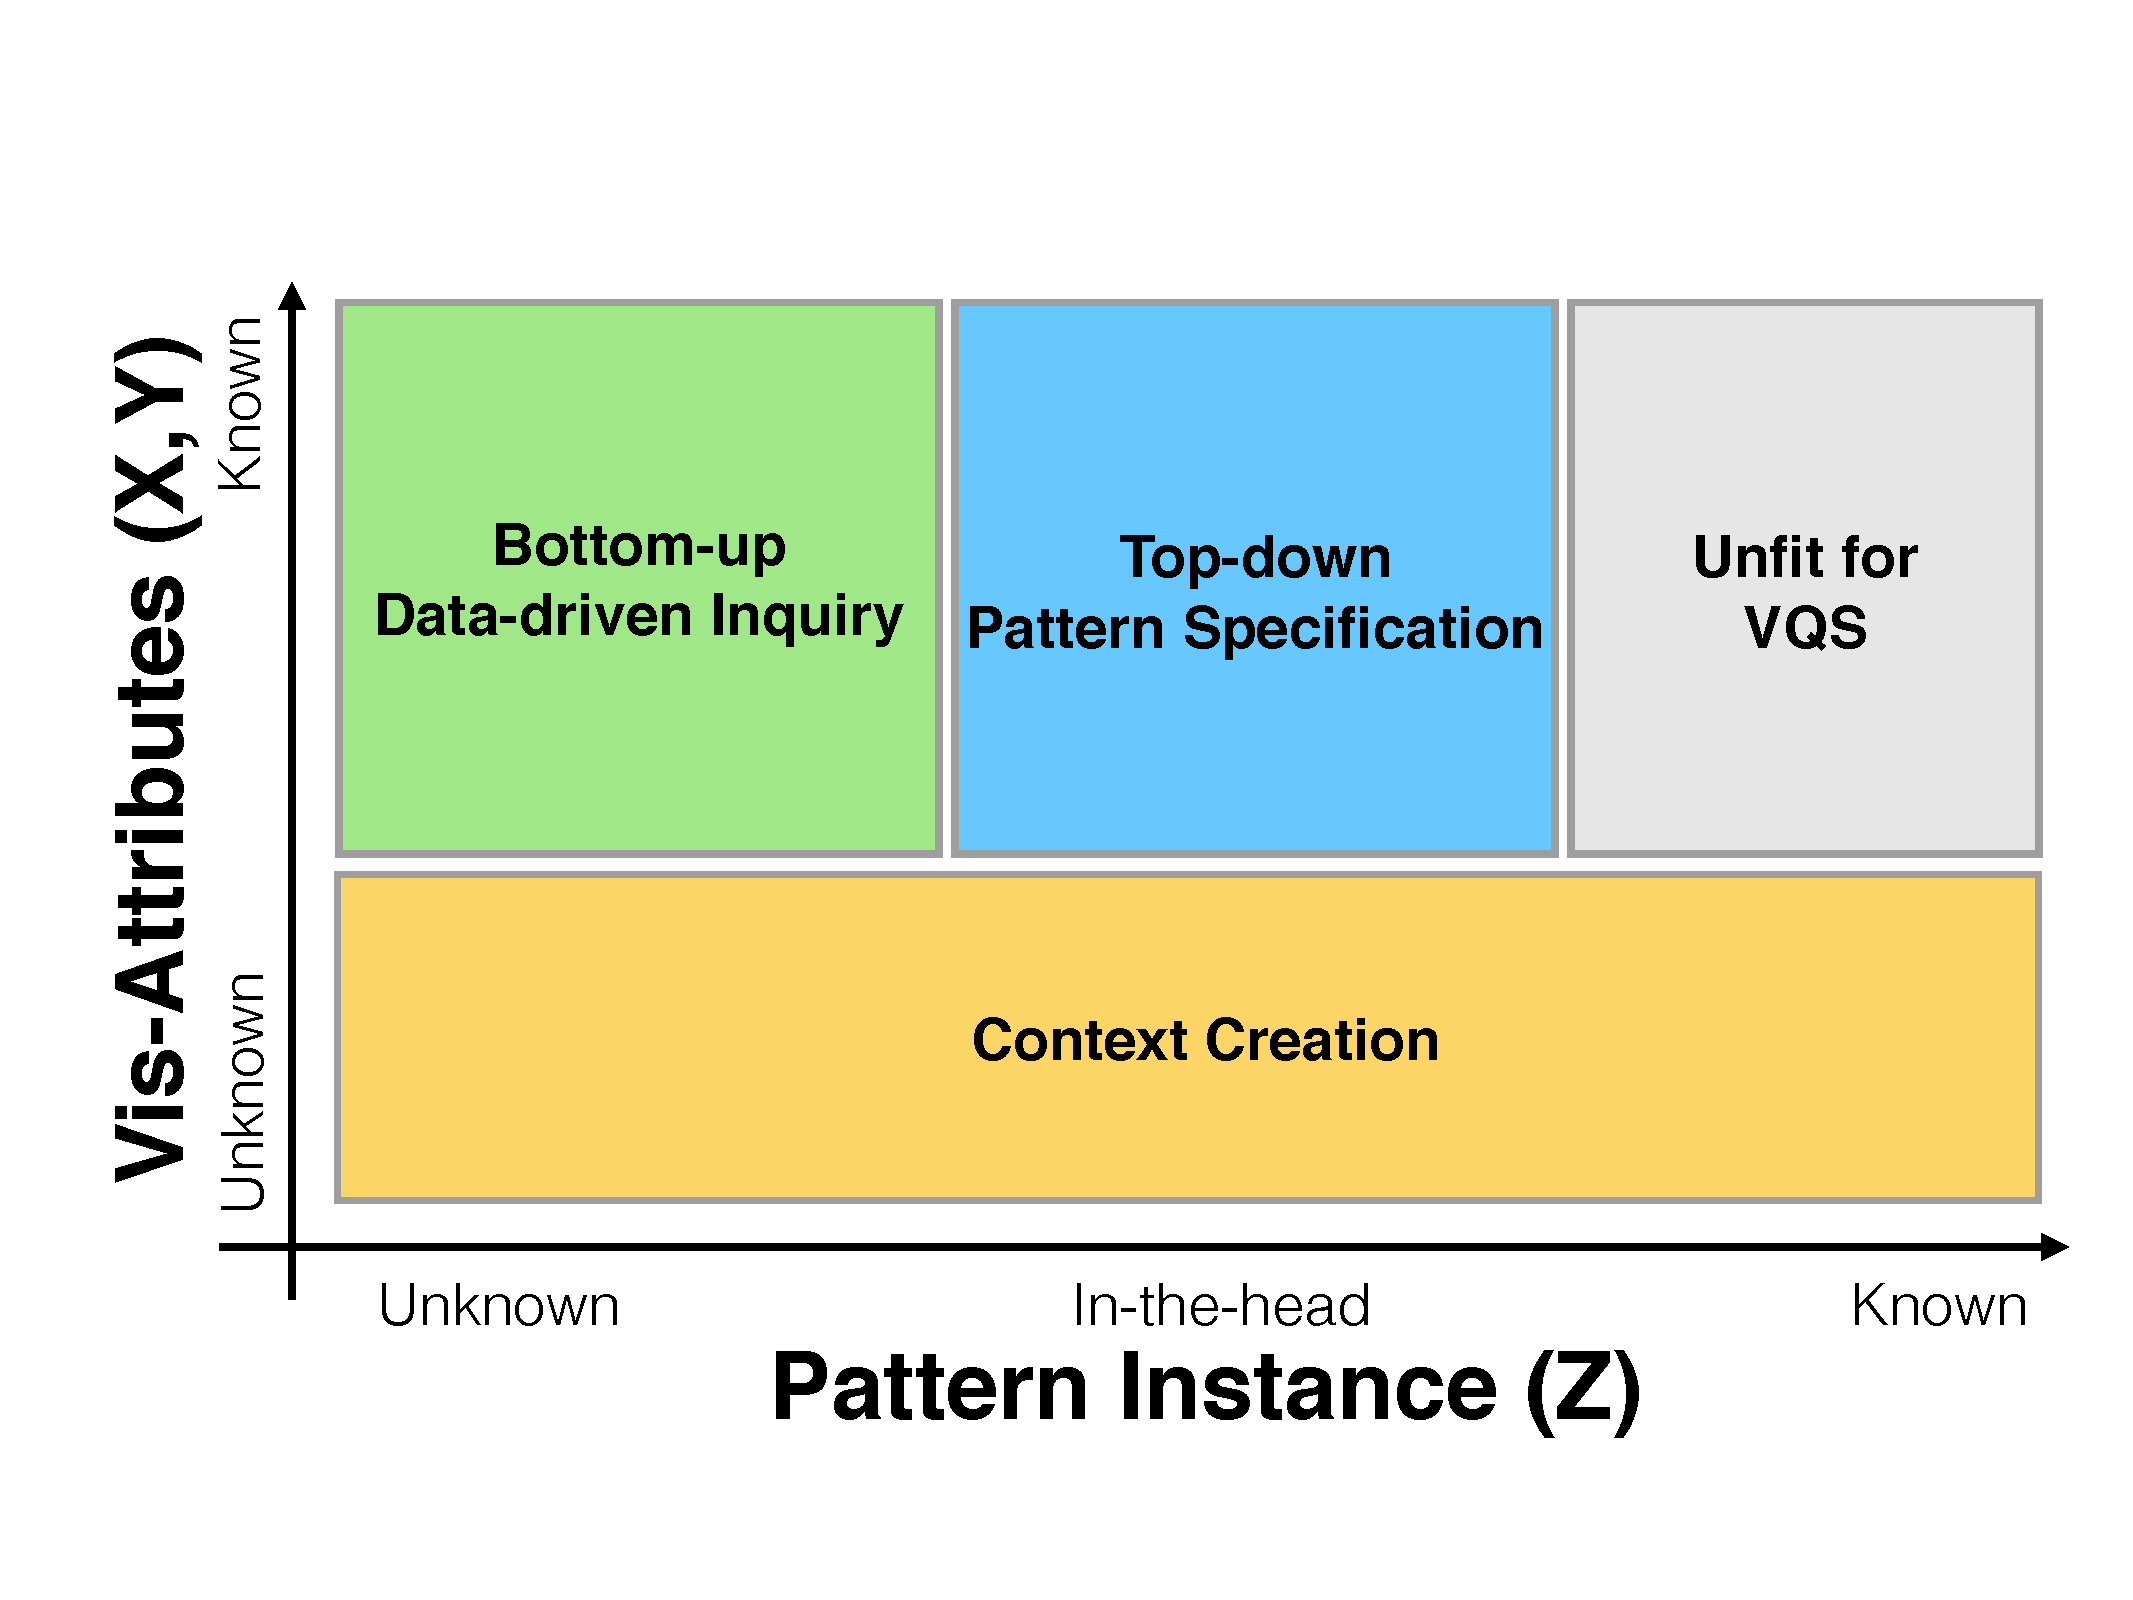
\includegraphics[width=0.9\linewidth]{figures/2dmodel.pdf}
  \caption{The problem space for VQSs is characterized by how much the analyst knows about the visualized attributes and the pattern instance. Colored areas highlight the three sensemaking processes in VQSs for addressing these characteristic problems. While prior work has focused solely on use cases in the blue region, we envision opportunities for VQSs beyond this to a larger space of use cases covered by the yellow and green regions.}
  \label{2dmodel}
  \vspace{-10pt}
\end{figure}
\begin{figure*}[ht!]
  \centering
  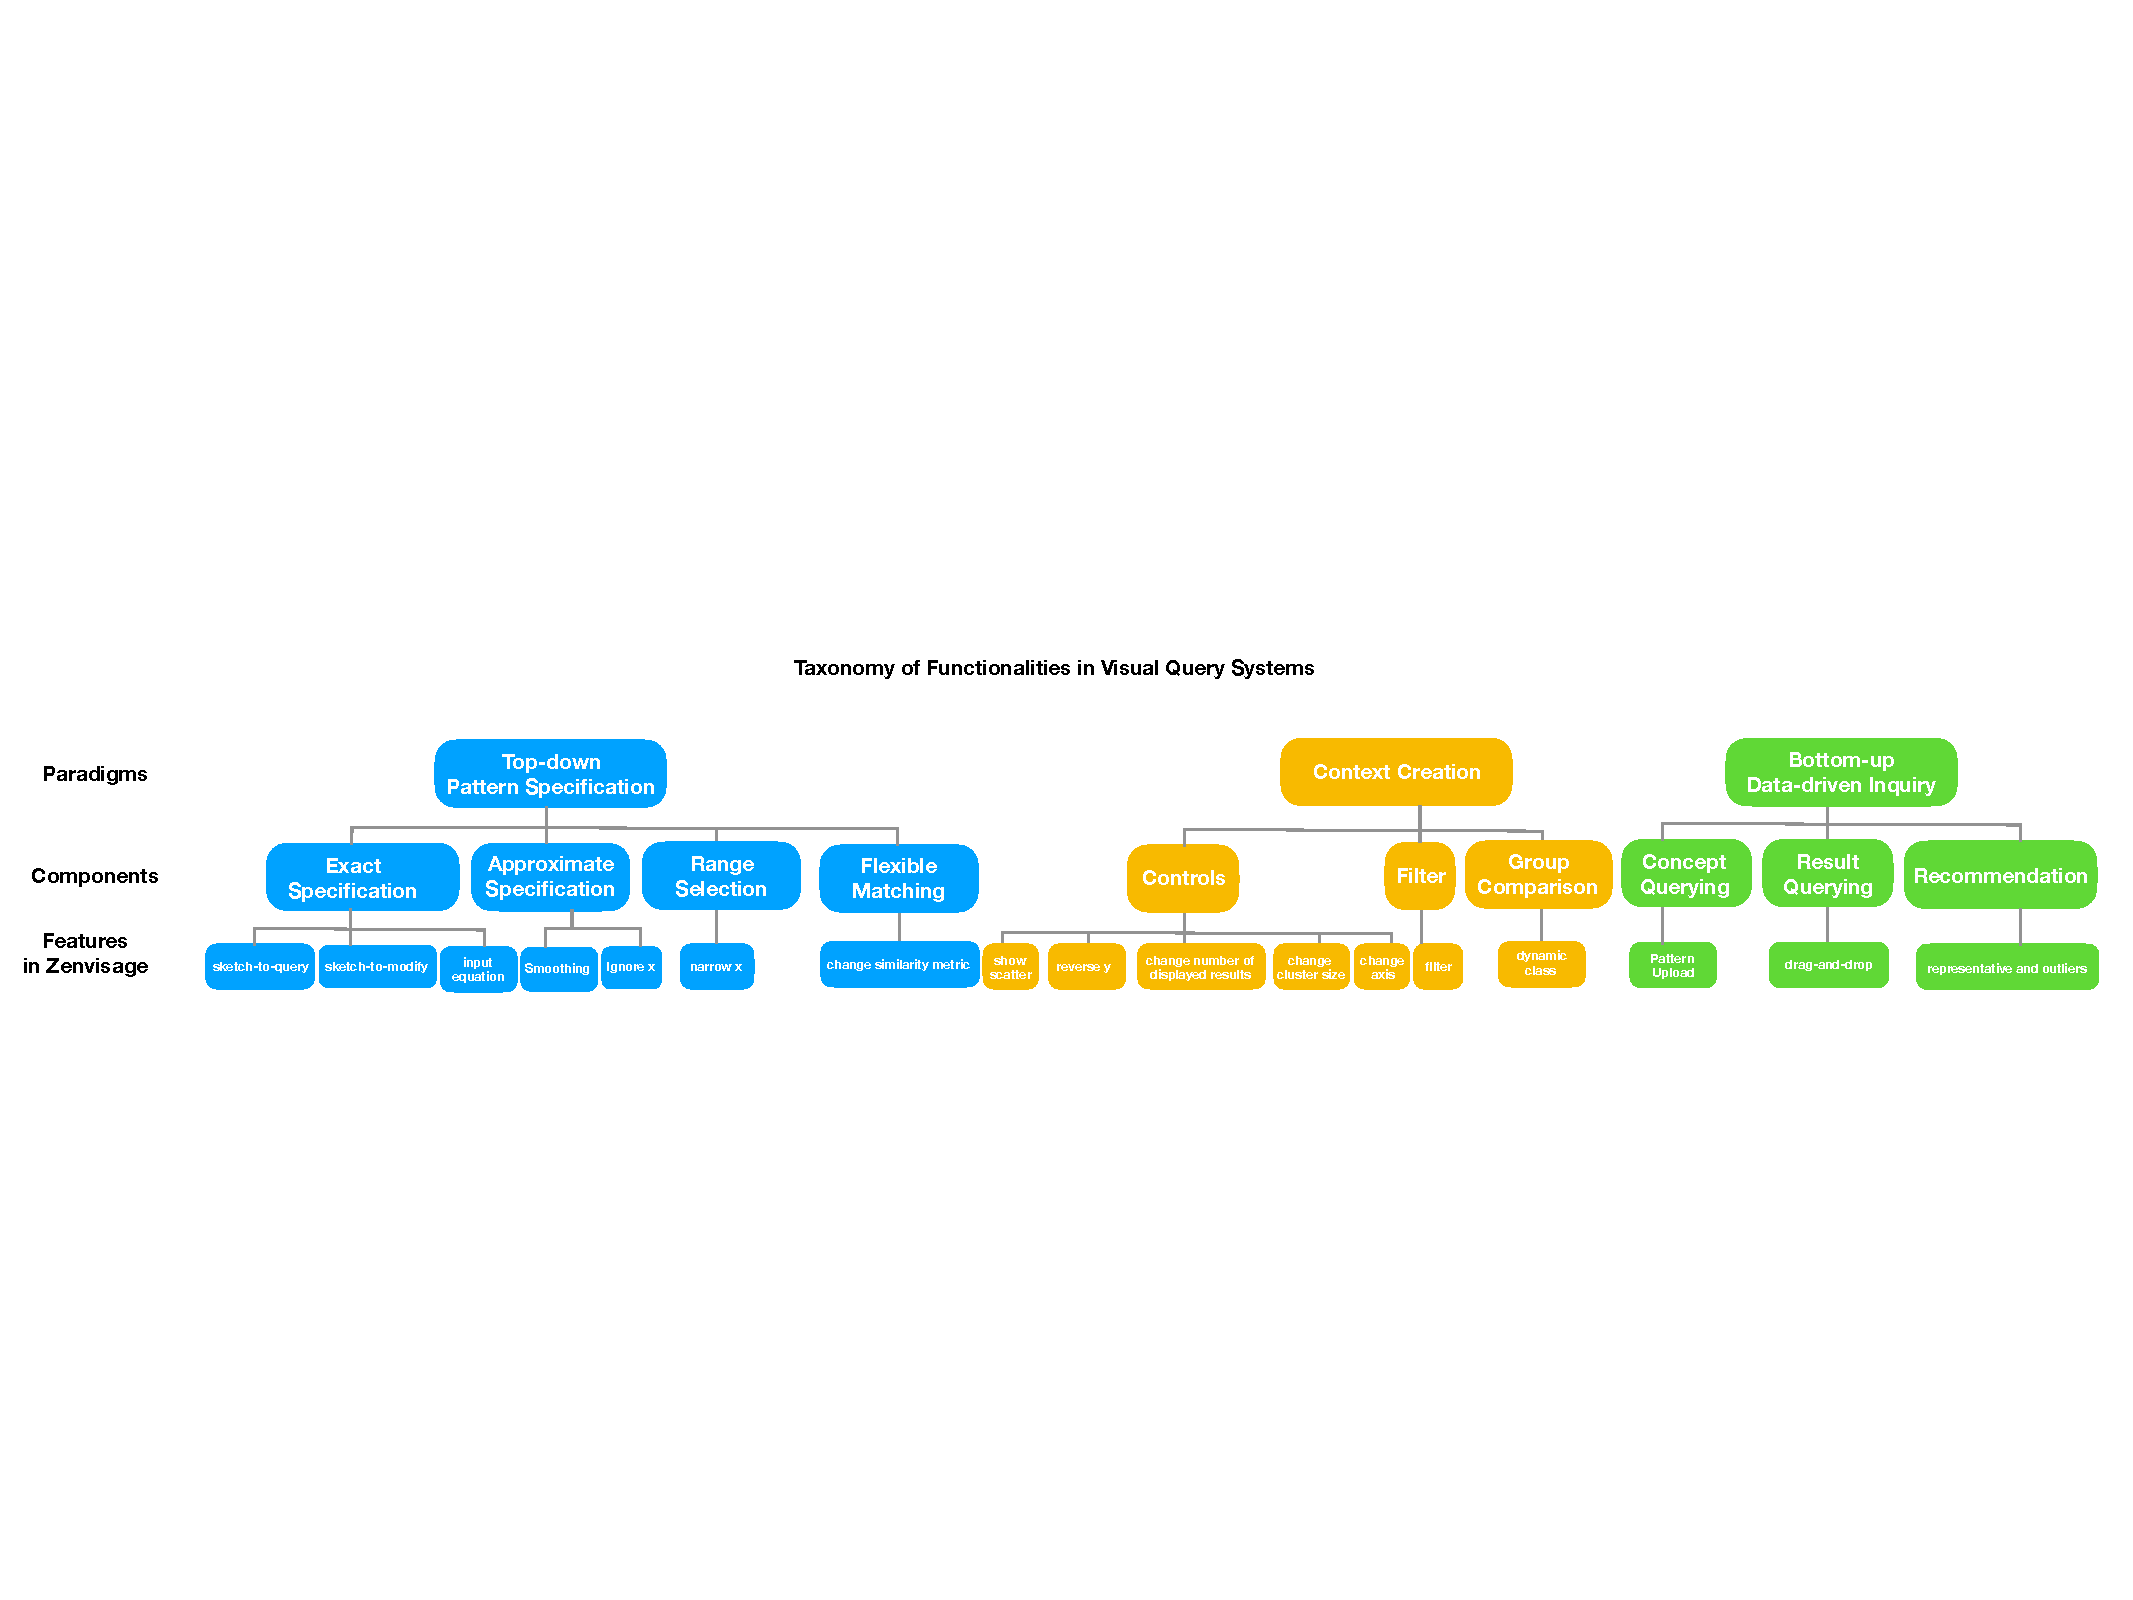
\includegraphics[width=0.9\linewidth]{figures/taxonomy.pdf}
  \caption{Taxonomy of \change{key capabilities essential to VQSs}. Each of the three sensemaking process is broken down into key functional components in VQSs. \change{Each component addresses a pro-forma question from a system's perspective.}} %, which is instantiated as features in \zvpp.}% The bottom-most layer connects the use cases features that have practical or envisioned usage based on the evaluation study.}
  \label{fig:taxonomy}
\end{figure*}
\change{
  \subsection{From Processes to Components: A VQS Taxonomy}
  After understanding how each sensemaking process fits into the problem space \change{addressable} by VQSs, we further explore design objectives of each sensemaking process, grounded in our collaborative design experience. Proceeding to the lower level of the Figure~\ref{fig:taxonomy} taxonomy, we then discuss how each sensemaking process is comprised of functional components that address challenges posed by the problem and dataset characteristics of each domain. Each of these VQS capabilities enable essential subtasks in accomplishing our participant's scientific goal, as exemplified in the usage scenarios in this section and further detailed in Appendix Table~\ref{bigfeaturetable}.
  \subsubsection{Top-Down Pattern Search}
  Top-down pattern search begins with the \change{analyst's} intuition about how the desired patterns should look like based on ``theory'', including visualizations from past experience or abstract conceptions based on external knowledge. The goal of top-down pattern search is to address the \textit{which} question of visual sensemaking: \textit{which \change{data instances exhibit} this pattern?} Based on this preconceived notion of what to search for, the design challenge is to translate the query \change{from} the analyst's head to a query executable by the VQS. This requires both components for specifying the pattern (\textit{pattern specification}), as well as controls governing the underlying algorithm of how shape-matching is performed (\textit{match specification}).
  %%%%%%%%%%%%%%%%%%%%%%%%Components%%%%%%%%%%%%%%%%%%%%%%%%%%%%
  \boldpara{Pattern Specification} interfaces allow users to submit exact descriptions of a pattern query. This is useful when the dataset contains \emph{large numbers of potentially-relevant pattern instances}.
  Since it is often difficult to sketch precisely, additional characteristics of the pattern query (e.g., patterns with specific shape characteristics, or expressible in a functional form) can be used to further winnow the list of undesired matches.%with the VQS returning a list of most similar matches
  \boldpara{Match Specification} addresses the well-known problem in VQSs where pattern queries are imprecise~\cite{correll2016semantics,Holz2009,Eichmann2015} by allowing users to clarifying how pattern matching should be performed. Match specification is useful when the dataset is \emph{noisy} (i.e., containing large numbers of false-positives). When the pattern query satisfies some additional constraints (e.g., pattern is x,y invariant), adjusting match specification prunes away false-positives to help reveal true candidates.
  \boldpara{Usage Scenario:} A1 knows based on a textbook definition of what a supernovae pattern should look like and the detailed shape characteristics, such as the amplitude of the peak and the level of error tolerance for defining a match. He can search for transient patterns through sketching, select the option to ignore differences along the temporal dimension, and change the similarity metric for flexible matching.
  \subsubsection{Context creation}
  \textit{Context creation} addresses the \textit{where} question of sensemaking by enabling analysts to navigate across different parts of the visualization collection to learn about \textit{where in the dataset do the patterns of interest lie}. The design challenge of context creation is to help users visualize and compare how data changes between different contexts by constructing different visualization collections via different visualization encodings (\textit{view specification} or different data subsets (\textit{slice-and-dice}).%to ensure that context is dynamically reflected across other VQS functionalities through
  %develop features that act as a `lens': navigating users to desired data subsets, visualizing and comparing how the data changes between the different lenses, and ensuring that context is dynamically reflected across other VQS functionalities.
  %%%%%%%%%%%%%%%%%%%%%%%%Components%%%%%%%%%%%%%%%%%%%%%%%%%%%%
  \boldpara{View specification} settings alter the encoding for all visualizations on the VQS. This ability to work with different collections of visualizations is useful when the dataset is \emph{multidimensional} and the axes of interest is \emph{unknown}. Modifying the view specification offers analysts different perspectives on the data to locate visualization collections of interest.
  \boldpara{Slice-and-Dice} empowers users to navigate and compare collections of visualizations constructed from different portions of the data. Data navigation capabilities is essential when the dataset has \emph{large numbers of non-visualized attributes} that may be related to the visualized attributes (e.g., geographical location may influence the time series pattern for housing prices). Analysts can either make use of pre-existing knowledge regarding these ``support attributes'' to navigate to a data region that is more likely to contain the desired pattern (e.g., filtering to suburbs to find cheaper housing) or discover unknown patterns and relationships between different data subsets (e.g., housing prices is lower in winter than compared to summer).% by gaining a better understanding of characteristic patterns in particular data region.
  \boldpara{Usage Scenario:} M1 recognizes salient trends in his dataset such as inverse or linear correlations, but does not have a pattern in mind to query with. Given a list of physical properties that he is interested in, he switches between different visualized attributes or dynamically creates different classes of data to examine the data from alternative perspectives.
  \subsubsection{Bottom-Up Data-Driven Inquiry}
  \textit{Bottom-up data-driven inquiry} is a browsing-oriented sensemaking process that goes from data to theory to
  addresses the \textit{what} questions in visual sensemaking: \textit{what are the patterns of interest in the dataset?} The design challenge include developing the right set of ``stimuli'' through \textit{recommendations} that could provoke further data-driven inquiries, as well as low-effort mechanisms to search via these results through \textit{result querying}.
  %%%%%%%%%%%%%%%%%%%%%%%%Components%%%%%%%%%%%%%%%%%%%%%%%%%%%%
  \boldpara{Recommendation} displays visualizations that may be of interest to users based on the current data context. Representative trends and outliers are useful for understanding common and outlying behaviors when a \emph{small number of common patterns} is exhibited in the dataset. %Understanding \emph{characteristic} patterns in dataset can help analysts discover other pattern queries of interest to jumpstart further queries.
  \boldpara{Result querying} enables users to query for patterns similar to a selected data pattern from the ranked list of results or recommendations. Typically, analyst select visualizations with \emph{semantic or visual properties} of interest and make use of results querying to understand characteristic properties of similar instances.
  \boldpara{Usage Scenario:} G2 does not have a preconceived knowledge of what to search for in the dataset. She is interested in learning about the characteristic patterns that exist in the dataset through representative trends, as a means to jumpstart further queries, as well as to understand groups of data instances with shared characteristics.
  \par The three aforementioned sensemaking processes are akin to the well-studied sensemaking paradigms of search, browse, and faceted navigation on the Web~\cite{Hearst2009,Olston2003}. Due to each of their advantages and limitations given different information seeking tasks, search interfaces have been designed to support all three complementary acts and transition smoothly between them to combine the strength of all three paradigms. \change{Similarly for VQSs, our design objective is to enable all the three sensemaking in \zvpp. As we discover in the Section~\ref{sec:eval_findings} evaluation study, this integrative approach not only accelerates the process of visualization discovery, but also encourages hypotheses generation and experimentation.}
}

% \change{
%   \subsection{Problems Addressed by Functional Components\label{sec:component}}
%     Here, we discuss how each functional component in the lower-level of our Figure~\ref{fig:taxonomy} taxonomy address specific challenges posed by the problem and dataset characteristics from each domain. Each of these VQS capabilities enable essential subtasks in accomplishing our participant's scientific  goal, as detailed in Appendix Table~\ref{bigfeaturetable}.
%     \boldpara{Pattern Specification} interfaces allow users to submit exact descriptions of a pattern query. This is useful when the dataset contains \emph{large numbers of potentially-relevant pattern instances}.
%     Since it is often difficult to sketch precisely, additional characteristics of the pattern query (e.g., patterns with specific shape characteristics, or expressible in a functional form) can be used to further winnow the list of undesired matches.%with the VQS returning a list of most similar matches
%     \boldpara{Match Specification} addresses the well-known problem in VQSs where pattern queries are imprecise~\cite{correll2016semantics,Holz2009,Eichmann2015} by allowing users to clarifying how pattern matching should be performed.
%     Match specification is useful when the dataset is \emph{noisy} (i.e., containing large numbers of false-positives). When the pattern query satisfies some additional constraints (e.g., pattern is x,y invariant), adjusting match specification prunes away false-positives to help reveal true candidates.
%     \boldpara{View specification} settings alter the encoding for all visualizations on the VQS. This ability to work with different collections of visualizations is useful when the dataset is \emph{multidimensional} and the axes of interest is \emph{unknown}. Modifying the view specification offers analysts different perspectives on the data to locate visualization collections of interest.
%     \boldpara{Slice-and-Dice} empowers users to navigate and compare collections of visualizations constructed from different portions of the data. Slice-and-dice is useful when the dataset has \emph{large numbers of non-visualized attributes} that may be related to the visualized attributes (e.g., geographical location may influence the time series pattern for housing prices). Analysts can either make use of pre-existing knowledge regarding these ``support attributes'' to navigate to a data region that is more likely to contain the desired pattern (e.g., filtering to suburbs to find cheaper housing) or discover unknown patterns and relationships between different data subsets (e.g., housing prices is lower in winter than compared to summer).% by gaining a better understanding of characteristic patterns in particular data region.
%     \boldpara{Result querying} enables users to query for patterns similar to a selected data pattern from the ranked list of results or recommendation. Typically, analyst select visualizations with \emph{semantic or visual properties} of interest and make use of results querying to understand characteristic properties of similar instances.
%     \boldpara{Recommendation} displays visualizations that may be of interest to users based on the data context. Representative trends and outliers are useful when a \emph{small number of common patterns} is exhibited in the dataset. Understanding \emph{characteristic} patterns in dataset can help analysts discover other pattern queries of interest to jumpstart further queries.
%   % % In this section, we first describe a model to help characterize the design space for VQS based on the analytical workload and usage patterns from different use cases. Then, we present design challenges related to each of the process.
% }
